% Options for packages loaded elsewhere
\PassOptionsToPackage{unicode}{hyperref}
\PassOptionsToPackage{hyphens}{url}
\PassOptionsToPackage{dvipsnames,svgnames,x11names}{xcolor}
%
\documentclass[
  letterpaper,
  DIV=11,
  numbers=noendperiod,
  oneside]{scrartcl}

\usepackage{amsmath,amssymb}
\usepackage{iftex}
\ifPDFTeX
  \usepackage[T1]{fontenc}
  \usepackage[utf8]{inputenc}
  \usepackage{textcomp} % provide euro and other symbols
\else % if luatex or xetex
  \usepackage{unicode-math}
  \defaultfontfeatures{Scale=MatchLowercase}
  \defaultfontfeatures[\rmfamily]{Ligatures=TeX,Scale=1}
\fi
\usepackage{lmodern}
\ifPDFTeX\else  
    % xetex/luatex font selection
\fi
% Use upquote if available, for straight quotes in verbatim environments
\IfFileExists{upquote.sty}{\usepackage{upquote}}{}
\IfFileExists{microtype.sty}{% use microtype if available
  \usepackage[]{microtype}
  \UseMicrotypeSet[protrusion]{basicmath} % disable protrusion for tt fonts
}{}
\makeatletter
\@ifundefined{KOMAClassName}{% if non-KOMA class
  \IfFileExists{parskip.sty}{%
    \usepackage{parskip}
  }{% else
    \setlength{\parindent}{0pt}
    \setlength{\parskip}{6pt plus 2pt minus 1pt}}
}{% if KOMA class
  \KOMAoptions{parskip=half}}
\makeatother
\usepackage{xcolor}
\usepackage[left=1in,marginparwidth=2.0666666666667in,textwidth=4.1333333333333in,marginparsep=0.3in]{geometry}
\setlength{\emergencystretch}{3em} % prevent overfull lines
\setcounter{secnumdepth}{-\maxdimen} % remove section numbering
% Make \paragraph and \subparagraph free-standing
\ifx\paragraph\undefined\else
  \let\oldparagraph\paragraph
  \renewcommand{\paragraph}[1]{\oldparagraph{#1}\mbox{}}
\fi
\ifx\subparagraph\undefined\else
  \let\oldsubparagraph\subparagraph
  \renewcommand{\subparagraph}[1]{\oldsubparagraph{#1}\mbox{}}
\fi

\usepackage{color}
\usepackage{fancyvrb}
\newcommand{\VerbBar}{|}
\newcommand{\VERB}{\Verb[commandchars=\\\{\}]}
\DefineVerbatimEnvironment{Highlighting}{Verbatim}{commandchars=\\\{\}}
% Add ',fontsize=\small' for more characters per line
\usepackage{framed}
\definecolor{shadecolor}{RGB}{241,243,245}
\newenvironment{Shaded}{\begin{snugshade}}{\end{snugshade}}
\newcommand{\AlertTok}[1]{\textcolor[rgb]{0.68,0.00,0.00}{#1}}
\newcommand{\AnnotationTok}[1]{\textcolor[rgb]{0.37,0.37,0.37}{#1}}
\newcommand{\AttributeTok}[1]{\textcolor[rgb]{0.40,0.45,0.13}{#1}}
\newcommand{\BaseNTok}[1]{\textcolor[rgb]{0.68,0.00,0.00}{#1}}
\newcommand{\BuiltInTok}[1]{\textcolor[rgb]{0.00,0.23,0.31}{#1}}
\newcommand{\CharTok}[1]{\textcolor[rgb]{0.13,0.47,0.30}{#1}}
\newcommand{\CommentTok}[1]{\textcolor[rgb]{0.37,0.37,0.37}{#1}}
\newcommand{\CommentVarTok}[1]{\textcolor[rgb]{0.37,0.37,0.37}{\textit{#1}}}
\newcommand{\ConstantTok}[1]{\textcolor[rgb]{0.56,0.35,0.01}{#1}}
\newcommand{\ControlFlowTok}[1]{\textcolor[rgb]{0.00,0.23,0.31}{#1}}
\newcommand{\DataTypeTok}[1]{\textcolor[rgb]{0.68,0.00,0.00}{#1}}
\newcommand{\DecValTok}[1]{\textcolor[rgb]{0.68,0.00,0.00}{#1}}
\newcommand{\DocumentationTok}[1]{\textcolor[rgb]{0.37,0.37,0.37}{\textit{#1}}}
\newcommand{\ErrorTok}[1]{\textcolor[rgb]{0.68,0.00,0.00}{#1}}
\newcommand{\ExtensionTok}[1]{\textcolor[rgb]{0.00,0.23,0.31}{#1}}
\newcommand{\FloatTok}[1]{\textcolor[rgb]{0.68,0.00,0.00}{#1}}
\newcommand{\FunctionTok}[1]{\textcolor[rgb]{0.28,0.35,0.67}{#1}}
\newcommand{\ImportTok}[1]{\textcolor[rgb]{0.00,0.46,0.62}{#1}}
\newcommand{\InformationTok}[1]{\textcolor[rgb]{0.37,0.37,0.37}{#1}}
\newcommand{\KeywordTok}[1]{\textcolor[rgb]{0.00,0.23,0.31}{#1}}
\newcommand{\NormalTok}[1]{\textcolor[rgb]{0.00,0.23,0.31}{#1}}
\newcommand{\OperatorTok}[1]{\textcolor[rgb]{0.37,0.37,0.37}{#1}}
\newcommand{\OtherTok}[1]{\textcolor[rgb]{0.00,0.23,0.31}{#1}}
\newcommand{\PreprocessorTok}[1]{\textcolor[rgb]{0.68,0.00,0.00}{#1}}
\newcommand{\RegionMarkerTok}[1]{\textcolor[rgb]{0.00,0.23,0.31}{#1}}
\newcommand{\SpecialCharTok}[1]{\textcolor[rgb]{0.37,0.37,0.37}{#1}}
\newcommand{\SpecialStringTok}[1]{\textcolor[rgb]{0.13,0.47,0.30}{#1}}
\newcommand{\StringTok}[1]{\textcolor[rgb]{0.13,0.47,0.30}{#1}}
\newcommand{\VariableTok}[1]{\textcolor[rgb]{0.07,0.07,0.07}{#1}}
\newcommand{\VerbatimStringTok}[1]{\textcolor[rgb]{0.13,0.47,0.30}{#1}}
\newcommand{\WarningTok}[1]{\textcolor[rgb]{0.37,0.37,0.37}{\textit{#1}}}

\providecommand{\tightlist}{%
  \setlength{\itemsep}{0pt}\setlength{\parskip}{0pt}}\usepackage{longtable,booktabs,array}
\usepackage{calc} % for calculating minipage widths
% Correct order of tables after \paragraph or \subparagraph
\usepackage{etoolbox}
\makeatletter
\patchcmd\longtable{\par}{\if@noskipsec\mbox{}\fi\par}{}{}
\makeatother
% Allow footnotes in longtable head/foot
\IfFileExists{footnotehyper.sty}{\usepackage{footnotehyper}}{\usepackage{footnote}}
\makesavenoteenv{longtable}
\usepackage{graphicx}
\makeatletter
\def\maxwidth{\ifdim\Gin@nat@width>\linewidth\linewidth\else\Gin@nat@width\fi}
\def\maxheight{\ifdim\Gin@nat@height>\textheight\textheight\else\Gin@nat@height\fi}
\makeatother
% Scale images if necessary, so that they will not overflow the page
% margins by default, and it is still possible to overwrite the defaults
% using explicit options in \includegraphics[width, height, ...]{}
\setkeys{Gin}{width=\maxwidth,height=\maxheight,keepaspectratio}
% Set default figure placement to htbp
\makeatletter
\def\fps@figure{htbp}
\makeatother
\newlength{\cslhangindent}
\setlength{\cslhangindent}{1.5em}
\newlength{\csllabelwidth}
\setlength{\csllabelwidth}{3em}
\newlength{\cslentryspacingunit} % times entry-spacing
\setlength{\cslentryspacingunit}{\parskip}
\newenvironment{CSLReferences}[2] % #1 hanging-ident, #2 entry spacing
 {% don't indent paragraphs
  \setlength{\parindent}{0pt}
  % turn on hanging indent if param 1 is 1
  \ifodd #1
  \let\oldpar\par
  \def\par{\hangindent=\cslhangindent\oldpar}
  \fi
  % set entry spacing
  \setlength{\parskip}{#2\cslentryspacingunit}
 }%
 {}
\usepackage{calc}
\newcommand{\CSLBlock}[1]{#1\hfill\break}
\newcommand{\CSLLeftMargin}[1]{\parbox[t]{\csllabelwidth}{#1}}
\newcommand{\CSLRightInline}[1]{\parbox[t]{\linewidth - \csllabelwidth}{#1}\break}
\newcommand{\CSLIndent}[1]{\hspace{\cslhangindent}#1}

\KOMAoption{captions}{tableheading}
\makeatletter
\makeatother
\makeatletter
\makeatother
\makeatletter
\@ifpackageloaded{caption}{}{\usepackage{caption}}
\AtBeginDocument{%
\ifdefined\contentsname
  \renewcommand*\contentsname{Table of contents}
\else
  \newcommand\contentsname{Table of contents}
\fi
\ifdefined\listfigurename
  \renewcommand*\listfigurename{List of Figures}
\else
  \newcommand\listfigurename{List of Figures}
\fi
\ifdefined\listtablename
  \renewcommand*\listtablename{List of Tables}
\else
  \newcommand\listtablename{List of Tables}
\fi
\ifdefined\figurename
  \renewcommand*\figurename{Figure}
\else
  \newcommand\figurename{Figure}
\fi
\ifdefined\tablename
  \renewcommand*\tablename{Table}
\else
  \newcommand\tablename{Table}
\fi
}
\@ifpackageloaded{float}{}{\usepackage{float}}
\floatstyle{ruled}
\@ifundefined{c@chapter}{\newfloat{codelisting}{h}{lop}}{\newfloat{codelisting}{h}{lop}[chapter]}
\floatname{codelisting}{Listing}
\newcommand*\listoflistings{\listof{codelisting}{List of Listings}}
\makeatother
\makeatletter
\@ifpackageloaded{caption}{}{\usepackage{caption}}
\@ifpackageloaded{subcaption}{}{\usepackage{subcaption}}
\makeatother
\makeatletter
\@ifpackageloaded{tcolorbox}{}{\usepackage[skins,breakable]{tcolorbox}}
\makeatother
\makeatletter
\@ifundefined{shadecolor}{\definecolor{shadecolor}{rgb}{.97, .97, .97}}
\makeatother
\makeatletter
\makeatother
\makeatletter
\@ifpackageloaded{sidenotes}{}{\usepackage{sidenotes}}
\@ifpackageloaded{marginnote}{}{\usepackage{marginnote}}
\makeatother
\makeatletter
\makeatother
\ifLuaTeX
  \usepackage{selnolig}  % disable illegal ligatures
\fi
\IfFileExists{bookmark.sty}{\usepackage{bookmark}}{\usepackage{hyperref}}
\IfFileExists{xurl.sty}{\usepackage{xurl}}{} % add URL line breaks if available
\urlstyle{same} % disable monospaced font for URLs
\hypersetup{
  pdftitle={A geographical statistical approach to the 2018 New Zealand Index of Multiple Deprevation},
  pdfauthor={Alice Clauss (260945446)},
  colorlinks=true,
  linkcolor={blue},
  filecolor={Maroon},
  citecolor={Blue},
  urlcolor={Blue},
  pdfcreator={LaTeX via pandoc}}

\title{A geographical statistical approach to the 2018 New Zealand Index
of Multiple Deprevation}
\usepackage{etoolbox}
\makeatletter
\providecommand{\subtitle}[1]{% add subtitle to \maketitle
  \apptocmd{\@title}{\par {\large #1 \par}}{}{}
}
\makeatother
\subtitle{GEOG 351: Quantitative Analysis}
\author{Alice Clauss (260945446)}
\date{2023-04-20}

\begin{document}
\maketitle
\ifdefined\Shaded\renewenvironment{Shaded}{\begin{tcolorbox}[sharp corners, borderline west={3pt}{0pt}{shadecolor}, interior hidden, frame hidden, boxrule=0pt, breakable, enhanced]}{\end{tcolorbox}}\fi

View the source code for this project
\href{https://github.com/legallyahc/geog351-finalproject}{here}.

\hypertarget{introduction}{%
\subsection{Introduction}\label{introduction}}

This paper ventures to investigate the links between education, mode of
transportation to work, and Maori status to multiple deprivation in New
Zealand. Greater active transportation to school has been linked to
higher rates of material and social deprivation in Quebec (Cutumisu et
al. 2014). Thus, I believe that greater use of active transportation
(such as cycling and public transit use) will be linked to a more
deprivation. Furthermore, increased car usage can indiciate a greater
lever of affluence (due to the money required for maintenance and gas),
leading to my prediction that greater private car usage will lead to
lower deprivation. In the literature, deprivation is typically used as a
predictor of educational attainment, rather than education determining
deprivation (Cooper, Lloyd-Reason, and Wall 2003; Shuttleworth 1995).
However, I believe that education and deprivation exhibit a positive
feedback (i.e.~as educational attainment decreases, material deprivation
increases, which decreases educational attainment), and thus chose to
investigate to what degree educational attainment influences
deprivation. In New Zealand, ethnic-density of Maori has been shown to
have a protective effect on health, but this is concealed by the impact
of the higher rates of deprivation that Maori experience (Bécares,
Cormack, and Harris 2013). I wanted to confirm the close link between
Maori status and deprivation already established in the literature as
well as see if this could be mitigated by education and mode of
transportation. With my focus on mode of transport, education, and Maori
status, I would like to see how well they predict deprivation and which
predictors are most influential. As deprivation is often spatially
autocorreleated, I will investigate if this holds for New Zealand
(Bécares, Cormack, and Harris 2013).

\hypertarget{methods}{%
\subsection{Methods}\label{methods}}

\hypertarget{data-sources}{%
\subsubsection{Data sources}\label{data-sources}}

\begin{Shaded}
\begin{Highlighting}[]
\FunctionTok{library}\NormalTok{(tidyverse)}
\NormalTok{imd18 }\OtherTok{\textless{}{-}}\NormalTok{ readxl}\SpecialCharTok{::}\FunctionTok{read\_excel}\NormalTok{(}\StringTok{"IMD2018.xlsx"}\NormalTok{, }\AttributeTok{sheet =} \StringTok{"IMD18"}\NormalTok{) }\CommentTok{\# Import data}
\end{Highlighting}
\end{Shaded}

The 2018 New Zealand Index of Multiple Deprivation (IMD) is a weighted
index of deprivation as determined by measures of employment, income,
crime, housing, health, education, and access as seen in
Figure~\ref{fig-IMD} (Exeter et al. 2018). Each observation is a ``Data
zone'', which corresponds to the 2013 New Zealand Census Unit, and
ordinal level data displaying the relative rank among all Data zones. It
contains variables for ranking by each of these measures and different
computations of the IMD that exclude each category (e.g.~the IMD without
any of the education inputs). For my study I chose to use the Index of
Multiple Deprivation that excluded educational data to maintain
independence among my variables. It contains 6181 unique observations.

\begin{Shaded}
\begin{Highlighting}[]
\CommentTok{\# Importing and cleaning education data}
\NormalTok{education }\OtherTok{\textless{}{-}} \FunctionTok{read\_csv}\NormalTok{(}\StringTok{"2018{-}census{-}place{-}summaries{-}csv/2018{-}census{-}place{-}summaries{-}education{-}table2{-}2018{-}csv.csv"}\NormalTok{) }\SpecialCharTok{\%\textgreater{}\%}
  \FunctionTok{filter}\NormalTok{(Area\_type }\SpecialCharTok{==} \StringTok{"Statistical Area 2"}\NormalTok{)}
\NormalTok{education }\OtherTok{\textless{}{-}}\NormalTok{ education }\SpecialCharTok{\%\textgreater{}\%}
  \FunctionTok{filter}\NormalTok{(Maori\_ethnic\_group\_indicator\_summary\_description }\SpecialCharTok{==} \StringTok{"Total"}\NormalTok{) }\SpecialCharTok{\%\textgreater{}\%}
  \FunctionTok{select}\NormalTok{(Year, Area\_type, Area\_code, Highest\_qualification\_description, Highest\_qualification\_percent) }\SpecialCharTok{\%\textgreater{}\%}
  \FunctionTok{pivot\_wider}\NormalTok{(}\AttributeTok{names\_from =}\NormalTok{ Highest\_qualification\_description, }\AttributeTok{values\_from =}\NormalTok{ Highest\_qualification\_percent) }\SpecialCharTok{\%\textgreater{}\%}
  \FunctionTok{select}\NormalTok{(}\SpecialCharTok{!}\FunctionTok{c}\NormalTok{(}\StringTok{\textasciigrave{}}\AttributeTok{Not elsewhere included}\StringTok{\textasciigrave{}}\NormalTok{, Total))}

\CommentTok{\# Importing and cleaning ethnicity data}
\NormalTok{ethnicity }\OtherTok{\textless{}{-}} \FunctionTok{read\_csv}\NormalTok{(}\StringTok{"2018{-}census{-}place{-}summaries{-}csv/2018{-}census{-}place{-}summaries{-}ethnicity{-}table1{-}2018{-}csv.csv"}\NormalTok{) }\SpecialCharTok{\%\textgreater{}\%}
  \FunctionTok{filter}\NormalTok{(Area\_type }\SpecialCharTok{==} \StringTok{"Statistical Area 2"}\NormalTok{)}
\NormalTok{ethnicity }\OtherTok{\textless{}{-}}\NormalTok{ ethnicity }\SpecialCharTok{\%\textgreater{}\%}
  \FunctionTok{select}\NormalTok{(Year, Area\_type, Area\_code, Maori\_descent\_description, Maori\_descent\_indicator\_percent) }\SpecialCharTok{\%\textgreater{}\%}
  \FunctionTok{pivot\_wider}\NormalTok{(}\AttributeTok{names\_from =}\NormalTok{ Maori\_descent\_description, }\AttributeTok{values\_from =}\NormalTok{ Maori\_descent\_indicator\_percent) }\SpecialCharTok{\%\textgreater{}\%}
  \FunctionTok{select}\NormalTok{(}\SpecialCharTok{!}\FunctionTok{c}\NormalTok{(}\StringTok{\textasciigrave{}}\AttributeTok{Response unidentifiable}\StringTok{\textasciigrave{}}\NormalTok{, }\StringTok{\textasciigrave{}}\AttributeTok{Not stated}\StringTok{\textasciigrave{}}\NormalTok{, }\StringTok{\textasciigrave{}}\AttributeTok{Total}\StringTok{\textasciigrave{}}\NormalTok{))}

\CommentTok{\# Cleaning transport data, spitting out the percentage of modes used for work, selecting SA2}
\NormalTok{transport }\OtherTok{\textless{}{-}} \FunctionTok{read\_csv}\NormalTok{(}\StringTok{"2018{-}census{-}place{-}summaries{-}csv/2018{-}census{-}place{-}summaries{-}transport{-}table1{-}2018{-}csv.csv"}\NormalTok{)}
\NormalTok{transport }\OtherTok{\textless{}{-}}\NormalTok{ transport }\SpecialCharTok{\%\textgreater{}\%}
  \FunctionTok{select}\NormalTok{(Year, Area\_type, Area\_code, }\StringTok{\textasciigrave{}}\AttributeTok{Main\_means\_of\_travel\_to\_work\_description}\StringTok{\textasciigrave{}}\NormalTok{, }\StringTok{\textasciigrave{}}\AttributeTok{Main\_means\_of\_travel\_to\_work\_percent}\StringTok{\textasciigrave{}}\NormalTok{) }\SpecialCharTok{\%\textgreater{}\%}
  \FunctionTok{pivot\_wider}\NormalTok{(}\AttributeTok{names\_from =} \StringTok{\textasciigrave{}}\AttributeTok{Main\_means\_of\_travel\_to\_work\_description}\StringTok{\textasciigrave{}}\NormalTok{, }\AttributeTok{values\_from =} \StringTok{\textasciigrave{}}\AttributeTok{Main\_means\_of\_travel\_to\_work\_percent}\StringTok{\textasciigrave{}}\NormalTok{) }\SpecialCharTok{\%\textgreater{}\%}
  \FunctionTok{filter}\NormalTok{(Area\_type }\SpecialCharTok{==} \StringTok{"Statistical Area 2"}\NormalTok{) }\SpecialCharTok{\%\textgreater{}\%}
  \FunctionTok{select}\NormalTok{(}\SpecialCharTok{!}\FunctionTok{c}\NormalTok{(}\StringTok{\textasciigrave{}}\AttributeTok{Did not go to work today}\StringTok{\textasciigrave{}}\NormalTok{, }\StringTok{\textasciigrave{}}\AttributeTok{Not elsewhere included}\StringTok{\textasciigrave{}}\NormalTok{))}

\CommentTok{\# Binding the census data together}
\NormalTok{vars }\OtherTok{\textless{}{-}} \FunctionTok{left\_join}\NormalTok{(education, ethnicity, }\AttributeTok{by =} \StringTok{"Area\_code"}\NormalTok{) }\SpecialCharTok{\%\textgreater{}\%}
  \FunctionTok{left\_join}\NormalTok{(., transport, }\AttributeTok{by =} \StringTok{"Area\_code"}\NormalTok{)}
\NormalTok{vars }\OtherTok{\textless{}{-}}\NormalTok{ vars }\SpecialCharTok{\%\textgreater{}\%}
  \FunctionTok{select}\NormalTok{(}\SpecialCharTok{!}\FunctionTok{c}\NormalTok{(Year, Year.y, Area\_type.y, Area\_type.x, Area\_type)) }\SpecialCharTok{\%\textgreater{}\%}
  \FunctionTok{rename}\NormalTok{(}
    \StringTok{\textasciigrave{}}\AttributeTok{Total Education}\StringTok{\textasciigrave{}} \OtherTok{=} \StringTok{\textasciigrave{}}\AttributeTok{Total stated.x}\StringTok{\textasciigrave{}}\NormalTok{,}
    \StringTok{\textasciigrave{}}\AttributeTok{Year}\StringTok{\textasciigrave{}} \OtherTok{=}\NormalTok{ Year.x,}
    \StringTok{\textasciigrave{}}\AttributeTok{Total Ethnicity}\StringTok{\textasciigrave{}} \OtherTok{=} \StringTok{\textasciigrave{}}\AttributeTok{Total stated.y}\StringTok{\textasciigrave{}}\NormalTok{,}
    \StringTok{\textasciigrave{}}\AttributeTok{Total Transport}\StringTok{\textasciigrave{}} \OtherTok{=} \StringTok{\textasciigrave{}}\AttributeTok{Total stated}\StringTok{\textasciigrave{}}
\NormalTok{  )}

\CommentTok{\# Creating groupings for education}
\NormalTok{vars }\OtherTok{\textless{}{-}}\NormalTok{ vars }\SpecialCharTok{\%\textgreater{}\%}
  \FunctionTok{mutate}\NormalTok{(}
    \AttributeTok{Secondary =} \FunctionTok{as.numeric}\NormalTok{(}\StringTok{\textasciigrave{}}\AttributeTok{Level 1 certificate}\StringTok{\textasciigrave{}}\NormalTok{) }\SpecialCharTok{+} \FunctionTok{as.numeric}\NormalTok{(}\StringTok{\textasciigrave{}}\AttributeTok{Level 2 certificate}\StringTok{\textasciigrave{}}\NormalTok{) }\SpecialCharTok{+} \FunctionTok{as.numeric}\NormalTok{(}\StringTok{\textasciigrave{}}\AttributeTok{Level 3 certificate}\StringTok{\textasciigrave{}}\NormalTok{) }\SpecialCharTok{+} \FunctionTok{as.numeric}\NormalTok{(}\StringTok{\textasciigrave{}}\AttributeTok{Overseas secondary school qualification}\StringTok{\textasciigrave{}}\NormalTok{),}
    \StringTok{\textasciigrave{}}\AttributeTok{Some University}\StringTok{\textasciigrave{}} \OtherTok{=} \FunctionTok{as.numeric}\NormalTok{(}\StringTok{\textasciigrave{}}\AttributeTok{Level 4 certificate}\StringTok{\textasciigrave{}}\NormalTok{) }\SpecialCharTok{+} \FunctionTok{as.numeric}\NormalTok{(}\StringTok{\textasciigrave{}}\AttributeTok{Level 5 diploma}\StringTok{\textasciigrave{}}\NormalTok{) }\SpecialCharTok{+} \FunctionTok{as.numeric}\NormalTok{(}\StringTok{\textasciigrave{}}\AttributeTok{Level 6 diploma}\StringTok{\textasciigrave{}}\NormalTok{),}
    \AttributeTok{Tertiary =} \FunctionTok{as.numeric}\NormalTok{(}\StringTok{\textasciigrave{}}\AttributeTok{Bachelor\textquotesingle{}s degree and level 7 qualification}\StringTok{\textasciigrave{}}\NormalTok{) }\SpecialCharTok{+} \FunctionTok{as.numeric}\NormalTok{(}\StringTok{\textasciigrave{}}\AttributeTok{Post{-}graduate and honours degrees}\StringTok{\textasciigrave{}}\NormalTok{),}
    \StringTok{\textasciigrave{}}\AttributeTok{Post{-}tertiary}\StringTok{\textasciigrave{}} \OtherTok{=} \FunctionTok{as.numeric}\NormalTok{(}\StringTok{\textasciigrave{}}\AttributeTok{Master\textquotesingle{}s degree}\StringTok{\textasciigrave{}}\NormalTok{) }\SpecialCharTok{+} \FunctionTok{as.numeric}\NormalTok{(}\StringTok{\textasciigrave{}}\AttributeTok{Doctorate degree}\StringTok{\textasciigrave{}}\NormalTok{),}
    \StringTok{\textasciigrave{}}\AttributeTok{Any University}\StringTok{\textasciigrave{}} \OtherTok{=} \FunctionTok{as.numeric}\NormalTok{(}\StringTok{\textasciigrave{}}\AttributeTok{Level 4 certificate}\StringTok{\textasciigrave{}}\NormalTok{) }\SpecialCharTok{+} \FunctionTok{as.numeric}\NormalTok{(}\StringTok{\textasciigrave{}}\AttributeTok{Level 5 diploma}\StringTok{\textasciigrave{}}\NormalTok{) }\SpecialCharTok{+} \FunctionTok{as.numeric}\NormalTok{(}\StringTok{\textasciigrave{}}\AttributeTok{Bachelor\textquotesingle{}s degree and level 7 qualification}\StringTok{\textasciigrave{}}\NormalTok{) }\SpecialCharTok{+} \FunctionTok{as.numeric}\NormalTok{(}\StringTok{\textasciigrave{}}\AttributeTok{Post{-}graduate and honours degrees}\StringTok{\textasciigrave{}}\NormalTok{) }\SpecialCharTok{+} \FunctionTok{as.numeric}\NormalTok{(}\StringTok{\textasciigrave{}}\AttributeTok{Master\textquotesingle{}s degree}\StringTok{\textasciigrave{}}\NormalTok{) }\SpecialCharTok{+} \FunctionTok{as.numeric}\NormalTok{(}\StringTok{\textasciigrave{}}\AttributeTok{Doctorate degree}\StringTok{\textasciigrave{}}\NormalTok{)}
\NormalTok{    ) }\SpecialCharTok{\%\textgreater{}\%}
  \FunctionTok{select}\NormalTok{(}\SpecialCharTok{!}\FunctionTok{c}\NormalTok{(}\StringTok{\textasciigrave{}}\AttributeTok{Level 1 certificate}\StringTok{\textasciigrave{}}\NormalTok{, }\StringTok{\textasciigrave{}}\AttributeTok{Level 2 certificate}\StringTok{\textasciigrave{}}\NormalTok{, }\StringTok{\textasciigrave{}}\AttributeTok{Level 3 certificate}\StringTok{\textasciigrave{}}\NormalTok{,}
            \StringTok{\textasciigrave{}}\AttributeTok{Level 4 certificate}\StringTok{\textasciigrave{}}\NormalTok{, }\StringTok{\textasciigrave{}}\AttributeTok{Level 5 diploma}\StringTok{\textasciigrave{}}\NormalTok{, }\StringTok{\textasciigrave{}}\AttributeTok{Level 6 diploma}\StringTok{\textasciigrave{}}\NormalTok{,}
            \StringTok{\textasciigrave{}}\AttributeTok{Bachelor\textquotesingle{}s degree and level 7 qualification}\StringTok{\textasciigrave{}}\NormalTok{, }\StringTok{\textasciigrave{}}\AttributeTok{Post{-}graduate and honours degrees}\StringTok{\textasciigrave{}}\NormalTok{,}
            \StringTok{\textasciigrave{}}\AttributeTok{Master\textquotesingle{}s degree}\StringTok{\textasciigrave{}}\NormalTok{, }\StringTok{\textasciigrave{}}\AttributeTok{Doctorate degree}\StringTok{\textasciigrave{}}\NormalTok{))}
\end{Highlighting}
\end{Shaded}

\marginnote{\begin{footnotesize}

New Zealand uses a unique method of classifying education attainment,
with a 7 level certificate / diploma system. I compiled this information
to be as comparable as possible to the Canadian system of ``Secondary'',
``Some University'', ``Bachelors'', ``Graduate'', and ``Post-graduate''.
I also combined these to make variables that combined any university
experience and any university degree past a Bachelors.

\end{footnotesize}}

To answer my research questions linking education, mode of transport,
and Maori status to deprivation, I used data from the 2018 New Zealand
Census at the Statistical Area 2 (SA2) geographic level (Stats NZ 2020).
Unfortunately, the SA2 zones are larger than the Data zones of the IMD,
with the census data having 2254 unique entries.

\begin{Shaded}
\begin{Highlighting}[]
\NormalTok{analysis }\OtherTok{\textless{}{-}} \FunctionTok{read\_csv}\NormalTok{(}\StringTok{"data.csv"}\NormalTok{) }\SpecialCharTok{\%\textgreater{}\%} 
  \FunctionTok{select}\NormalTok{(RnkIMDNoEd, No\_qual, Maori, Drive\_priv, Bus, Masters\_, AnyUni, Bicycle1) }\SpecialCharTok{\%\textgreater{}\%} 
  \FunctionTok{rename}\NormalTok{(}
    \AttributeTok{Bike =}\NormalTok{ Bicycle1}
\NormalTok{  )}
  \CommentTok{\# Import spatially joined data}
\end{Highlighting}
\end{Shaded}

To combine these two data sources, I used a spatial join in ArcGIS Pro
with the \emph{greatest overlap} method, joining the census data to the
IMD. This resulted in some of the resulting entries having the same
census data variables, but unique deprivation values, which lead to
inherent spatial correlation among these census variables. This resulted
in 6181 different observations in the final dataset.

\hypertarget{variables}{%
\subsubsection{Variables}\label{variables}}

\textbf{Response}

\texttt{RnkIMDNoEdu}: Ranked index of multiple deprivation that was made
without education data (Ordinal).

\textbf{Predictors}

\texttt{No\_qual}: \% of people with no proof of education (Ratio).

\texttt{AnyUni}: \% of people who have any university education (Ratio).

\texttt{Master\_}: \% of people with post-bachelor's education (Ratio).

\texttt{Maori}: \% of people with Maori heritage (Ratio).

\texttt{Drive\_priv}: \% of people who drive their own vehicle to work
(Ratio).

\texttt{Bus}: \% of people who take the bus to work (Ratio).

\texttt{Bike}: \% of people who bike to work (Ratio).

Only \texttt{No\_qual} and \texttt{AnyUni} appear to be normally
distributed, with \texttt{RnkIMDNoEdu} uniformly distributed,
\texttt{Master\_} right skewed, and \texttt{Drive\_priv} left skewed
(see Figure~\ref{fig-notransform}). While I would use a Shapiro-Wilk
test to confirm their lack of normality, it is invalid for samples with
\(> 5000\) observations.

\texttt{Bike}, \texttt{Bus}, and \texttt{Maori} appear to have a
logistic distribution and were thus transformed.

\begin{Shaded}
\begin{Highlighting}[]
\NormalTok{analysis }\OtherTok{\textless{}{-}}\NormalTok{ analysis }\SpecialCharTok{\%\textgreater{}\%}
  \FunctionTok{mutate}\NormalTok{(}
    \AttributeTok{log\_maori =} \FunctionTok{log}\NormalTok{(Maori),}
    \AttributeTok{log\_bus =} \FunctionTok{log}\NormalTok{(Bus),}
    \AttributeTok{log\_bike =} \FunctionTok{log}\NormalTok{(Bike)}
\NormalTok{  )}
  \CommentTok{\# Logarithmic transform on some variables}
\end{Highlighting}
\end{Shaded}

After this transformation, \texttt{Bike} and \texttt{Maori} appear more
normally distributed, while \texttt{Bus} has a very large number of
values at one point and is otherwise uniformly distributed (see
Figure~\ref{fig-transform}).

\hypertarget{analysis-methods}{%
\subsubsection{Analysis methods}\label{analysis-methods}}

All relationships will be investigated through a Spearman correlation
and a multiple linear regression model, with the potential spatial
correlation of multiple deprivation in New Zealand investigated through
Moran's I and, if significantly related, evaluated in a spatial multiple
linear regression model.

\hypertarget{spearman-correlation}{%
\paragraph{Spearman Correlation}\label{spearman-correlation}}

The Spearman Correlation is a non-parametric test of correlation,
requiring only that each sample is independent from each other. It
accepts Ordinal, Interval, and Ratio level data. It will be run on each
predictor variable and the response variable to assess the predictors'
correlation to the response and any potential collinearity. I also used
Bonferroni p-value correction to correct the significance value of any
of the many comparisons I made.

\hypertarget{multiple-linear-regression}{%
\paragraph{Multiple Linear
Regression}\label{multiple-linear-regression}}

The relationship between the variables will then be investigated with an
Ordinary Least Squares multiple linear regression, with the predictor
variables determining the response. This assumes that the relationship
is linear, the predictors are normally distributed, there is no
collinearity among the predictors, the residuals are homoskedastic, and
the residuals are normally distributed. We can ignore the requirement of
normality for the predictors due to the large number of observations and
will test our assumptions after the model.

\hypertarget{morans-i}{%
\paragraph{Moran's I}\label{morans-i}}

Moran's I investigates the spatial autocorrelation of a variable, with a
positive value indicating positive spatial autocorrelation. For this
dataset, \texttt{RnkIMDNoEd} will be investigated due to its lack of
duplication of variables and to answer our initial research question.

\hypertarget{spatial-multiple-linear-regression}{%
\paragraph{Spatial Multiple Linear
Regression}\label{spatial-multiple-linear-regression}}

The final multiple linear regression model will be run in GeoDa using a
Queen weights to test the significance of spatial lag and spatial error.
If both are significant, the more significant test will determine the
model to be run. For a spatial lag model, this means that a spatially
significant lag of our result variable is added to our predictors. For a
spatial error model, any potentially spatially dependent errors are
resolved.

\hypertarget{results-and-discussion}{%
\subsection{Results and discussion}\label{results-and-discussion}}

\hypertarget{spearman-correlation-1}{%
\subsubsection{Spearman Correlation}\label{spearman-correlation-1}}

\begin{Shaded}
\begin{Highlighting}[]
\KeywordTok{spearman}\NormalTok{ rnkimdnoed no\_qual drive\_priv log\_bus masters\_ anyuni log\_maori log\_bike, }\KeywordTok{stats}\NormalTok{(rho }\KeywordTok{obs} \KeywordTok{p}\NormalTok{) bonferroni}
\end{Highlighting}
\end{Shaded}

The results of the Spearman correlation are visible in
Figure~\ref{fig-spearmancorr}. As we can see from the STATA output, the
comparison is limited by the number of observations in \texttt{log\_bus}
(4669 observations). Every corresponding correlation is significant at
the 95\% confidence level aside from \texttt{log\_maori} and
\texttt{log\_bike}. However, \texttt{AnyUni} and \texttt{Master\_} have
a Pearson correlation of more than \(0.9\) with \texttt{No\_qual}, which
indicates that these variables are likely autocorrelated. As
\texttt{No\_qual} has the greatest correlation with \texttt{RnkIMDNoEd},
it will preserved while \texttt{AnyUni} and \texttt{Master\_} are
excluded from further analysis.

\marginnote{\begin{footnotesize}

After a logistic transformation any zero values receive a value of
\(-\infty\) and were thus excluded from analysis.

\end{footnotesize}}

From our Spearman correlation, we can conclude that a higher rate of no
of educational qualifications is related to a higher rate of
deprivation, while a greater amount of any university education is
correlated to a lower rate of deprivation. Somewhat confusingly, any
amount of university education is more correlated to a lower rate of
deprivation than only those with a graduate degree or beyond (Spearman
correlation coefficient of \(-0.5622\) to \(-0.5244\)). Maori status is
significantly related to a higher rate of deprivation with a coefficient
of \(0.6945\). In contrast to my original hypothesis, greater modal
share of driving a private vehicle to work is related to a higher rate
of deprivation (coefficient of \(0.3521\)). Active transportation (in
the form of riding a bike or taking a public bus) is linked to lower
rates of deprivation, with the log transform of these variables having a
correlation coefficient of \(-0.0472\) and \(-0.0792\) respectively.

\hypertarget{multiple-linear-regression-1}{%
\subsubsection{Multiple Linear
Regression}\label{multiple-linear-regression-1}}

\hypertarget{models}{%
\paragraph{Models}\label{models}}

\begin{Shaded}
\begin{Highlighting}[]
\KeywordTok{regress}\NormalTok{ rnkimdnoed no\_qual drive\_priv log\_bus log\_maori log\_bike, beta}
\KeywordTok{regress}\NormalTok{ rnkimdnoed no\_qual log\_bus log\_maori log\_bike, beta}
\KeywordTok{regress}\NormalTok{ rnkimdnoed no\_qual log\_bus log\_maori, beta}
\end{Highlighting}
\end{Shaded}

The initial regression model is visible at Figure~\ref{fig-ols1}. Here,
both \texttt{Drive\_priv} and \texttt{log\_bike} are not significant,
though \texttt{Drive\_priv} is more so, and was thus excluded from the
next model, visible in Figure~\ref{fig-ols2}. As \texttt{log\_bike}
still has an insignificant p-value, and was excluded. The final model,
visible in Figure~\ref{fig-ols3}, has an adjusted \(R^2\) of \(0.6156\)
and a \(\sqrt{MSE}\) of \(1118.6\). I believe that this is a reasonable
model for an ordinal response variable, with a relatively high \(R^2\)
though the \(\sqrt{MSE}\) is rather high because of the uniformly
distributed response variable.

\begin{longtable}[]{@{}ll@{}}
\toprule\noalign{}
Predictors & Beta Coefficients \\
\midrule\noalign{}
\endhead
\bottomrule\noalign{}
\endlastfoot
\texttt{no\_qual} & 0.4358954 \\
\texttt{log\_bus} & 0.3789292 \\
\texttt{log\_maori} & 0.5379429 \\
\end{longtable}

We can now consider the combined influence of mode of transport,
educational attainment, and Maori status on deprivation. Maori status
has the greatest effect on deprivation with a \(\beta\) coefficient of
\(0.54\), while a lack of educational qualifications is still
influential with a \(\beta\) coefficient of \(0.44\). Bus ridership to
work, while less important, is influential with a \(\beta\) coefficient
of \(0.38\). Unlike the Pearson correlation, however, an increase in bus
ridership is related to a greater rate of deprivation in the linear
regression model, but maintains my original prediction that greater
active transportation would be linked to higher rates of deprivation.

\hypertarget{assumptions}{%
\paragraph{Assumptions}\label{assumptions}}

\begin{Shaded}
\begin{Highlighting}[]
\KeywordTok{rvfplot}
\KeywordTok{estat} \KeywordTok{hettest}
\KeywordTok{vif}
\end{Highlighting}
\end{Shaded}

Even before testing our assumptions made of our multiple linear
regression model, we already know that our data was not normally
distributed prior to our analysis. This is confirmed by the Residuals
vs.~Fitted plot (Figure~\ref{fig-rvf}), which has a strong negative
linear trend due to the uniformity of the response variable.

However, the variance of the residuals must also be assessed. Using a
Breusch--Pagan/Cook--Weisberg test for heteroskedasticity, we reject the
null hypothesis of homoskedasticity and affirm that the residuals are
heteroskedastic (Figure~\ref{fig-hettest}).

We can confirm that there is no autocorrelation between our variables by
checking the Variance inflation factors (VIFs) of each independent
variable (Figure~\ref{fig-vif}), where the greatest value is \(2.18\)
for \texttt{No\_qual}.

\hypertarget{morans-i-1}{%
\subsubsection{Moran's I}\label{morans-i-1}}

Figure~\ref{fig-globali} displays the Global Moran's I scatter plot,
with an I of \(0.668\) using a Queen weights matrix for
\texttt{RnkIMDNoEd}. This has a p-value of 0.001 with 999 random
permutations (Figure~\ref{fig-moransig}), indicating that there is a
significant spatial correlation to deprivation in New Zealand. This is
visible in the local clusters of deprivation
(Figure~\ref{fig-localiclusters}), many of which are highly
statistically significant (Figure~\ref{fig-localisig}). Thus we can
confirm our hypothesis that deprivation in New Zealand is spatially
correlated.

\hypertarget{spatial-multiple-linear-regression-1}{%
\subsubsection{Spatial Multiple Linear
Regression}\label{spatial-multiple-linear-regression-1}}

Knowing that deprivation in New Zealand is spatially correlated, we can
improve our linear regression model. While running the previous
regression model in GeoDa produces a different output (as it does not
exclude the same values as STATA), the outputs of the spatial
correlation tests are still valid. Figure~\ref{fig-spatial} displays the
values and significance of the Lagrange multipliers for spatial lag and
spatial error, leading me to choose a spatial lag multiple linear
regression due to its greater Robust LM value (395, \(p=0.000\) to
Spatial Errror's 129, \(p=0.000\)).

The spatial lag multiple linear regression (Figure~\ref{fig-spatiallag})
was conducted with a Queen weight matrix with any isolates removed on
the same variables as the final multiple linear regression
(\texttt{No\_qual}, \texttt{log\_maori}, and \texttt{log\_bike}). The
spatial lag linear regression model has an \(R^2\) of \(0.705\) and a
\(\sqrt{MSE}\) of \(969\), considerable improvements from the standard
linear regression. However, the model is still heteroskedastic,
rejecting the null hypothesis of homoskedasticity in the Breusch-Pagan
test, nor are the residuals normally distributed. However, the model
does show the significant impact that the spatial distribution has on
deprivation in New Zealand, with each other predictor variable having a
z-value of \(\approx 22.5\).

\hypertarget{conclusions}{%
\subsection{Conclusions}\label{conclusions}}

Links to deprivation in New Zealand have been investigated before but
have taken the form of deprivation's impacts on other aspects of life.
Investigating potential linkages to deprivation can allow us to better
consider the patterns of who experience the most deprivation, which are
often those least able to cope with it. This investigation involved some
ad-hoc change of procedures, particularly in the linking of the 2018 New
Zealand Index of Multiple Deprivation and Census New Zealand's 2018 SA2
data. While the original 2013 IMD had the same geographic zones as the
2013 New Zealand Census, in 2018 New Zealand updated its census units
and structures to allow for more data to be available to researchers.
However, the 2018 IMD, to maintain continuity with the 2013 IMD, did not
change its geographic units. My oversight of these differences required
me to perform a spatial join in ArcGIS Pro, which was not the ideal way
to combine these datasets. With more time or experience using a Thiessen
polygon construction or Inverse Distance Weighting method to interpolate
the census data to the IMD data would have been ideal. With the linkage
of lack of educational credentials, bike usage, and Maori status to
deprivation, a deeper dive can be made into how these connections have
come to be or what mechanisms maintain them.

\hypertarget{appendix-1.-figures}{%
\subsection{Appendix 1. Figures}\label{appendix-1.-figures}}

\begin{figure}

{\centering 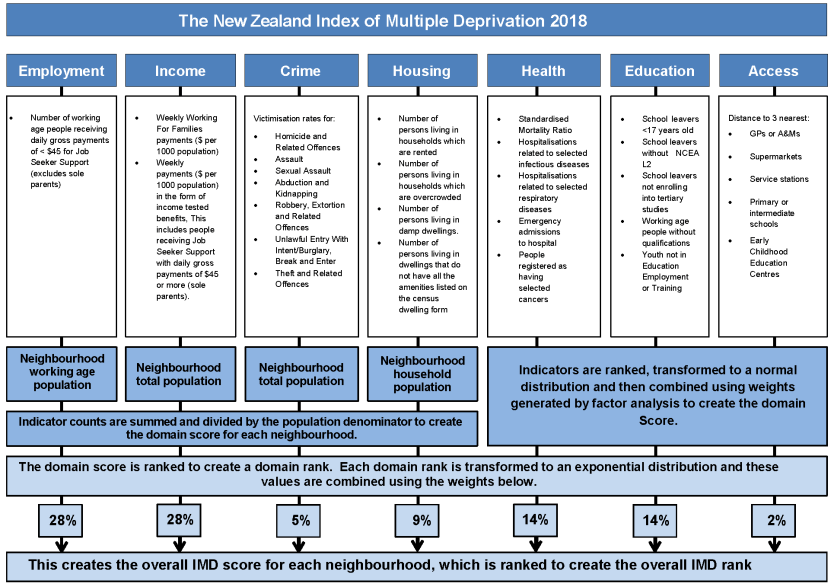
\includegraphics{final_pres_wrap/IMD_2018_development.png}

}

\caption{\label{fig-IMD}Weighting of the 2018 IMD (Exeter et al. 2018).}

\end{figure}

\begin{figure}

{\centering 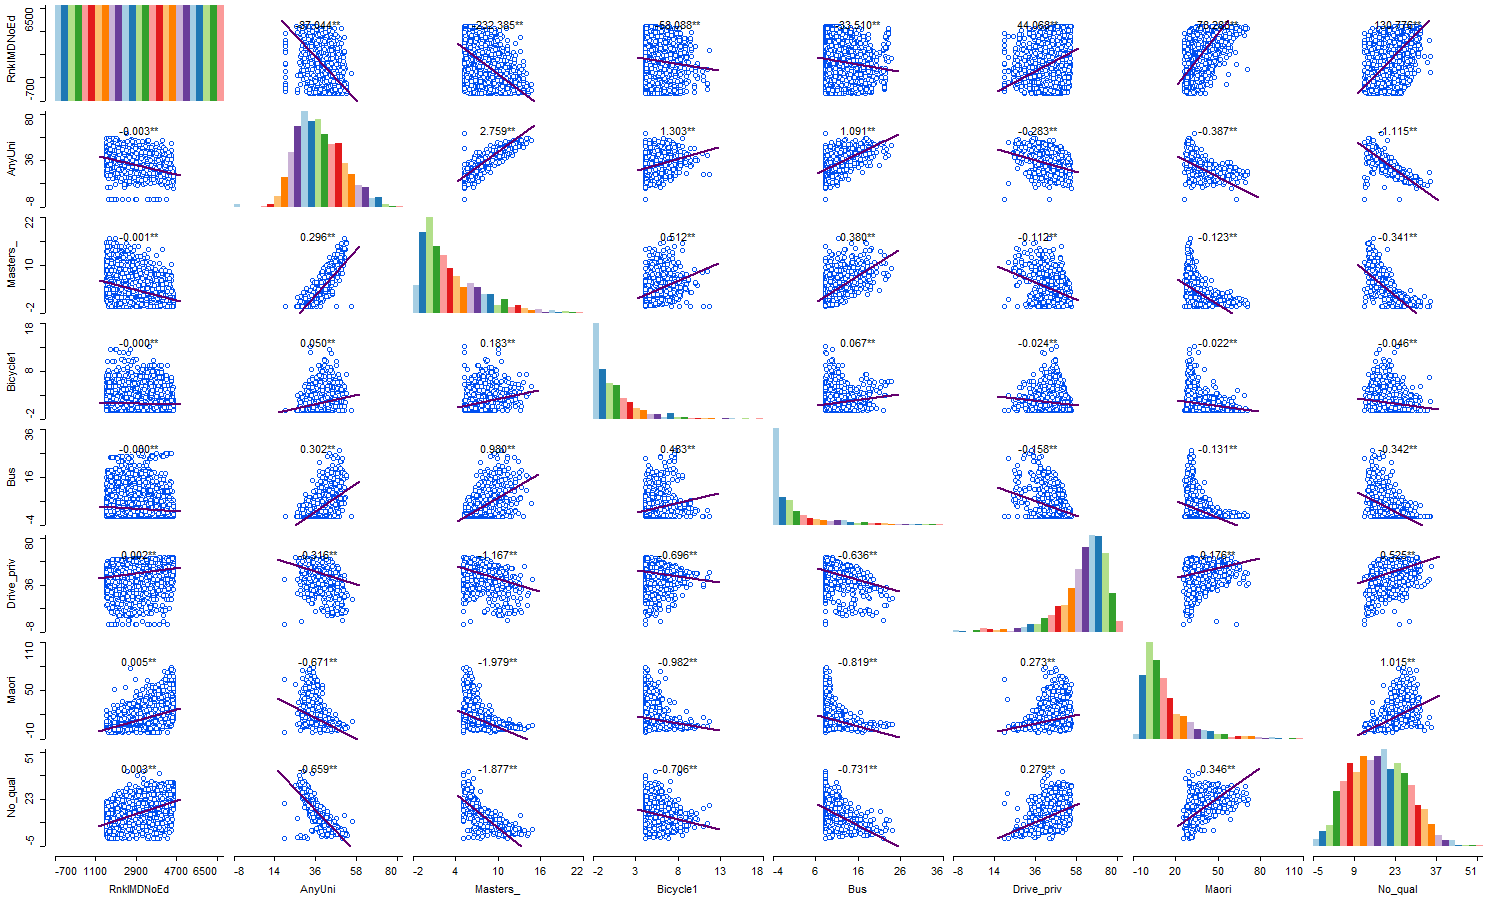
\includegraphics{scattermatrix_notransform.png}

}

\caption{\label{fig-notransform}Initial scatterplot and histogram matrix
for the selected variables. Please disregard the stated correlation
values.}

\end{figure}

\begin{figure}

{\centering 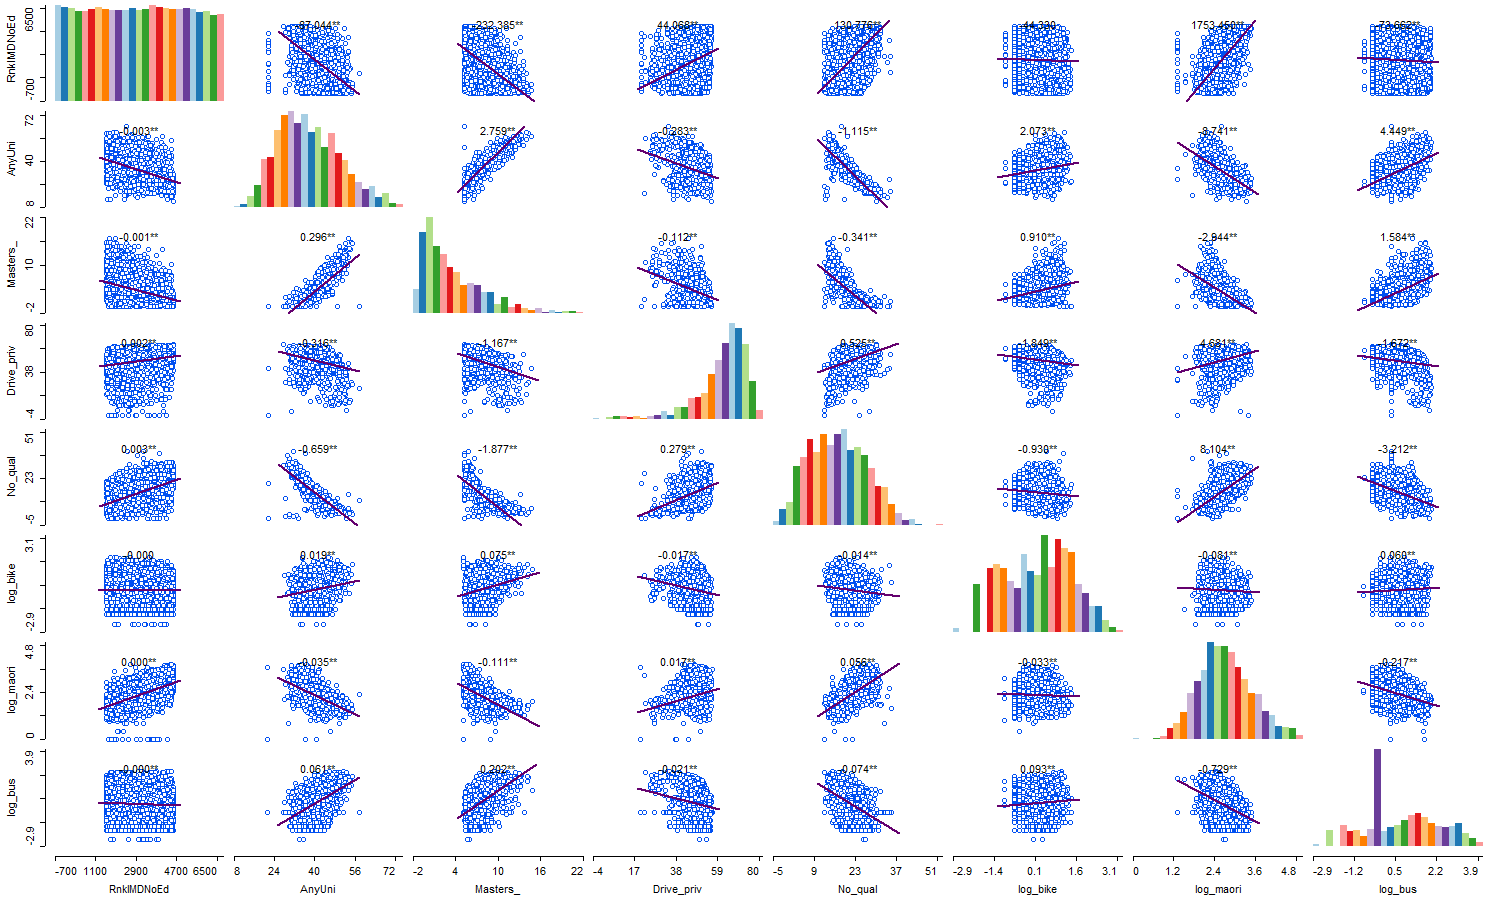
\includegraphics{scattermatrix_transformed.png}

}

\caption{\label{fig-transform}Transformed scatterplot and histogram
matrix, with the new distributions of \texttt{log\_bike},
\texttt{log\_maori}, and \texttt{log\_bus} appearing more normal.}

\end{figure}

\marginnote{\begin{footnotesize}

After transformation, \texttt{RnkIMDNoEd} is no longer normal. As some
entries for \texttt{maori}, \texttt{bike}, and \texttt{bus} were not
available (e.g.~\(-\infty\)), these entries were removed from the
dataset.

\end{footnotesize}}

\begin{figure}

{\centering 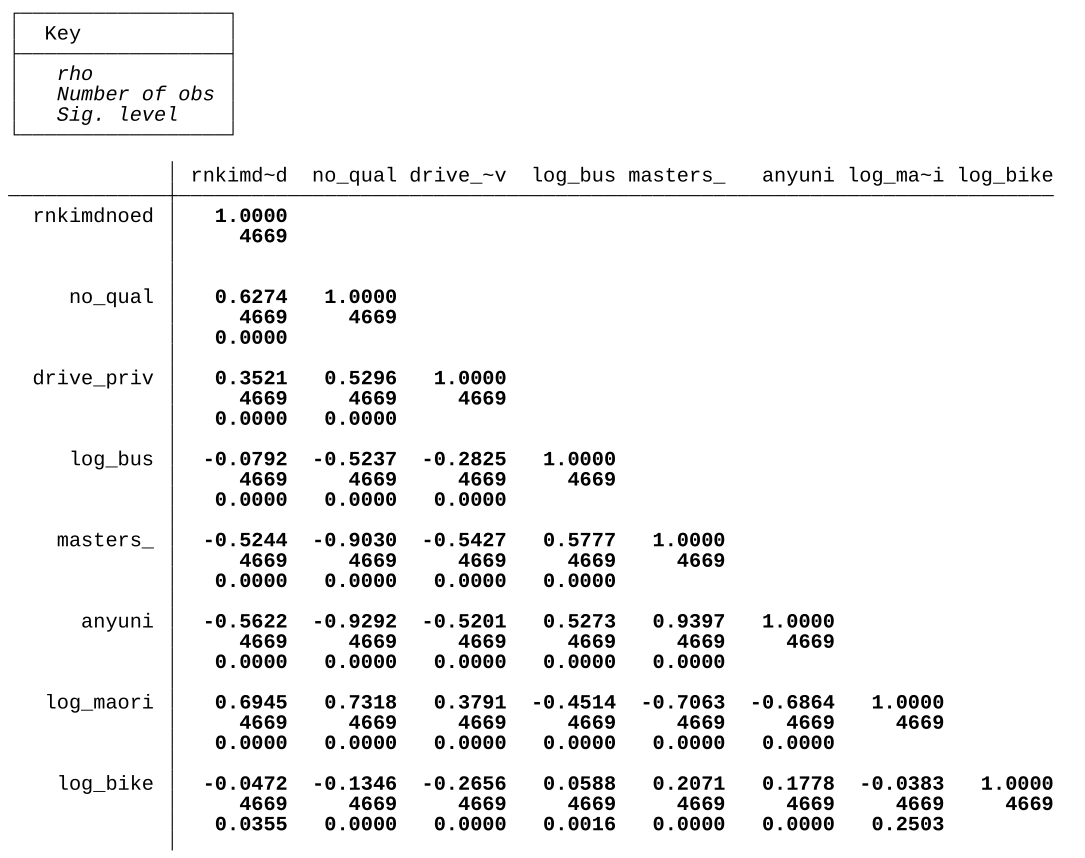
\includegraphics{Screenshot from 2023-04-20 06-24-16.png}

}

\caption{\label{fig-spearmancorr}Output of the Pearson correlation from
STATA. The key is included at the top left.}

\end{figure}

\begin{figure}

{\centering 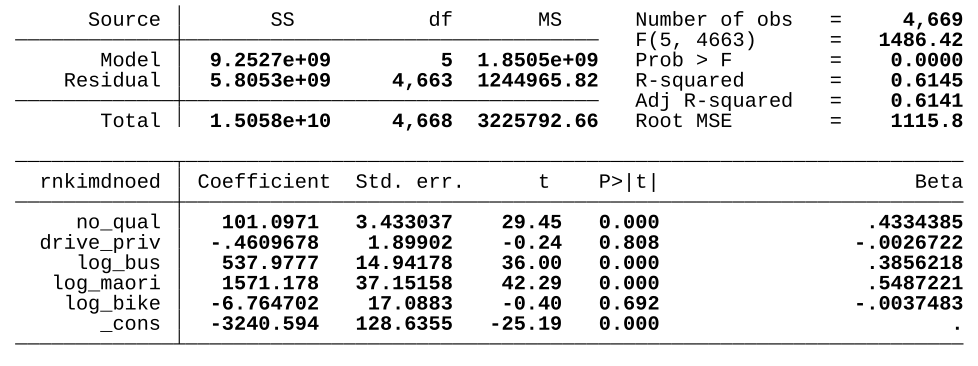
\includegraphics{Screenshot from 2023-04-20 06-49-02.png}

}

\caption{\label{fig-ols1}Output of the first multiple linear regression
in STATA.}

\end{figure}

\begin{figure}

{\centering 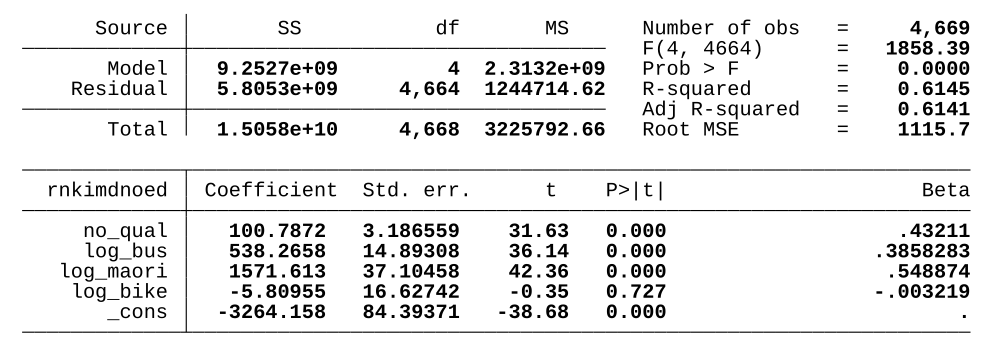
\includegraphics{Screenshot from 2023-04-20 06-52-56.png}

}

\caption{\label{fig-ols2}Output of the second multiple linear regression
STATA (\texttt{drive\_priv} removed).}

\end{figure}

\begin{figure}

{\centering 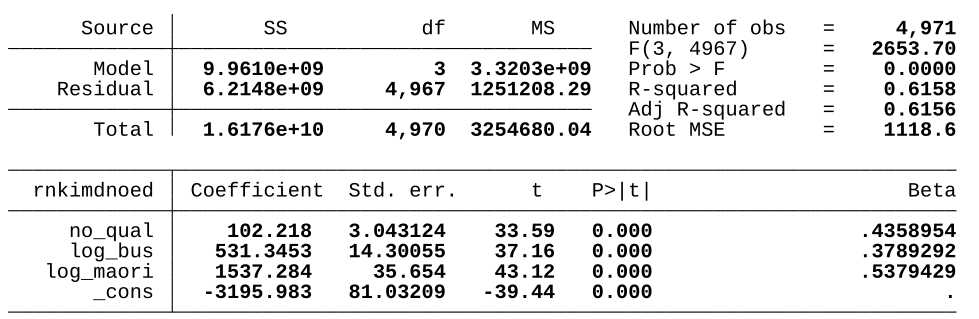
\includegraphics{Screenshot from 2023-04-20 06-53-21.png}

}

\caption{\label{fig-ols3}Output of the third multiple linear regression
in STATA (\texttt{log\_bike} removed).}

\end{figure}

\begin{figure}

{\centering 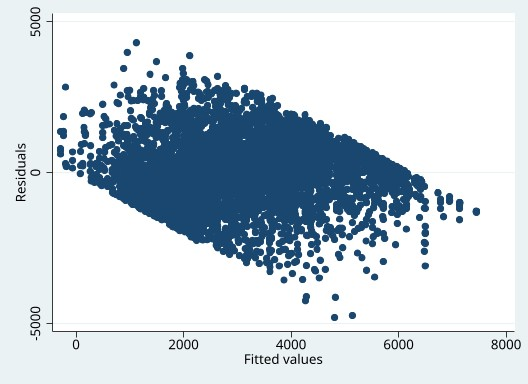
\includegraphics{rvfplot.jpg}

}

\caption{\label{fig-rvf}Residuals versus fitted values plot of the final
linear regression model.}

\end{figure}

\begin{figure}

{\centering 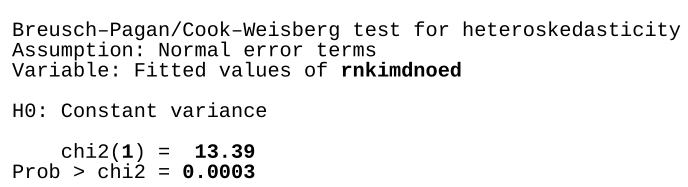
\includegraphics{hettest.png}

}

\caption{\label{fig-hettest}Results of the Breusch--Pagan/Cook--Weisberg
test for heteroskedasticity from STATA.}

\end{figure}

\begin{figure}

{\centering 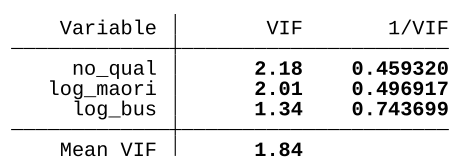
\includegraphics{vif.png}

}

\caption{\label{fig-vif}Variance inflation factor output of the final
linear regression model.}

\end{figure}

\begin{figure}

{\centering 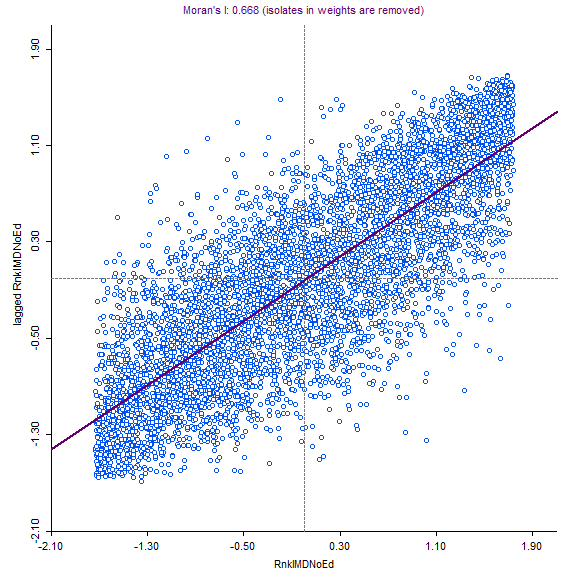
\includegraphics{imdnoed_globalmoranI_uni.png}

}

\caption{\label{fig-globali}Global Moran's I of \texttt{RnkIMDNoEd} from
Geoda.}

\end{figure}

\begin{figure}

{\centering \includegraphics{Global Moran\textquotesingle{}s I significance output.png}

}

\caption{\label{fig-moransig}Random significance testing output of the
Global Moran's I of \texttt{RnkIMDNoEd} from GeoDa.}

\end{figure}

\begin{figure}

{\centering 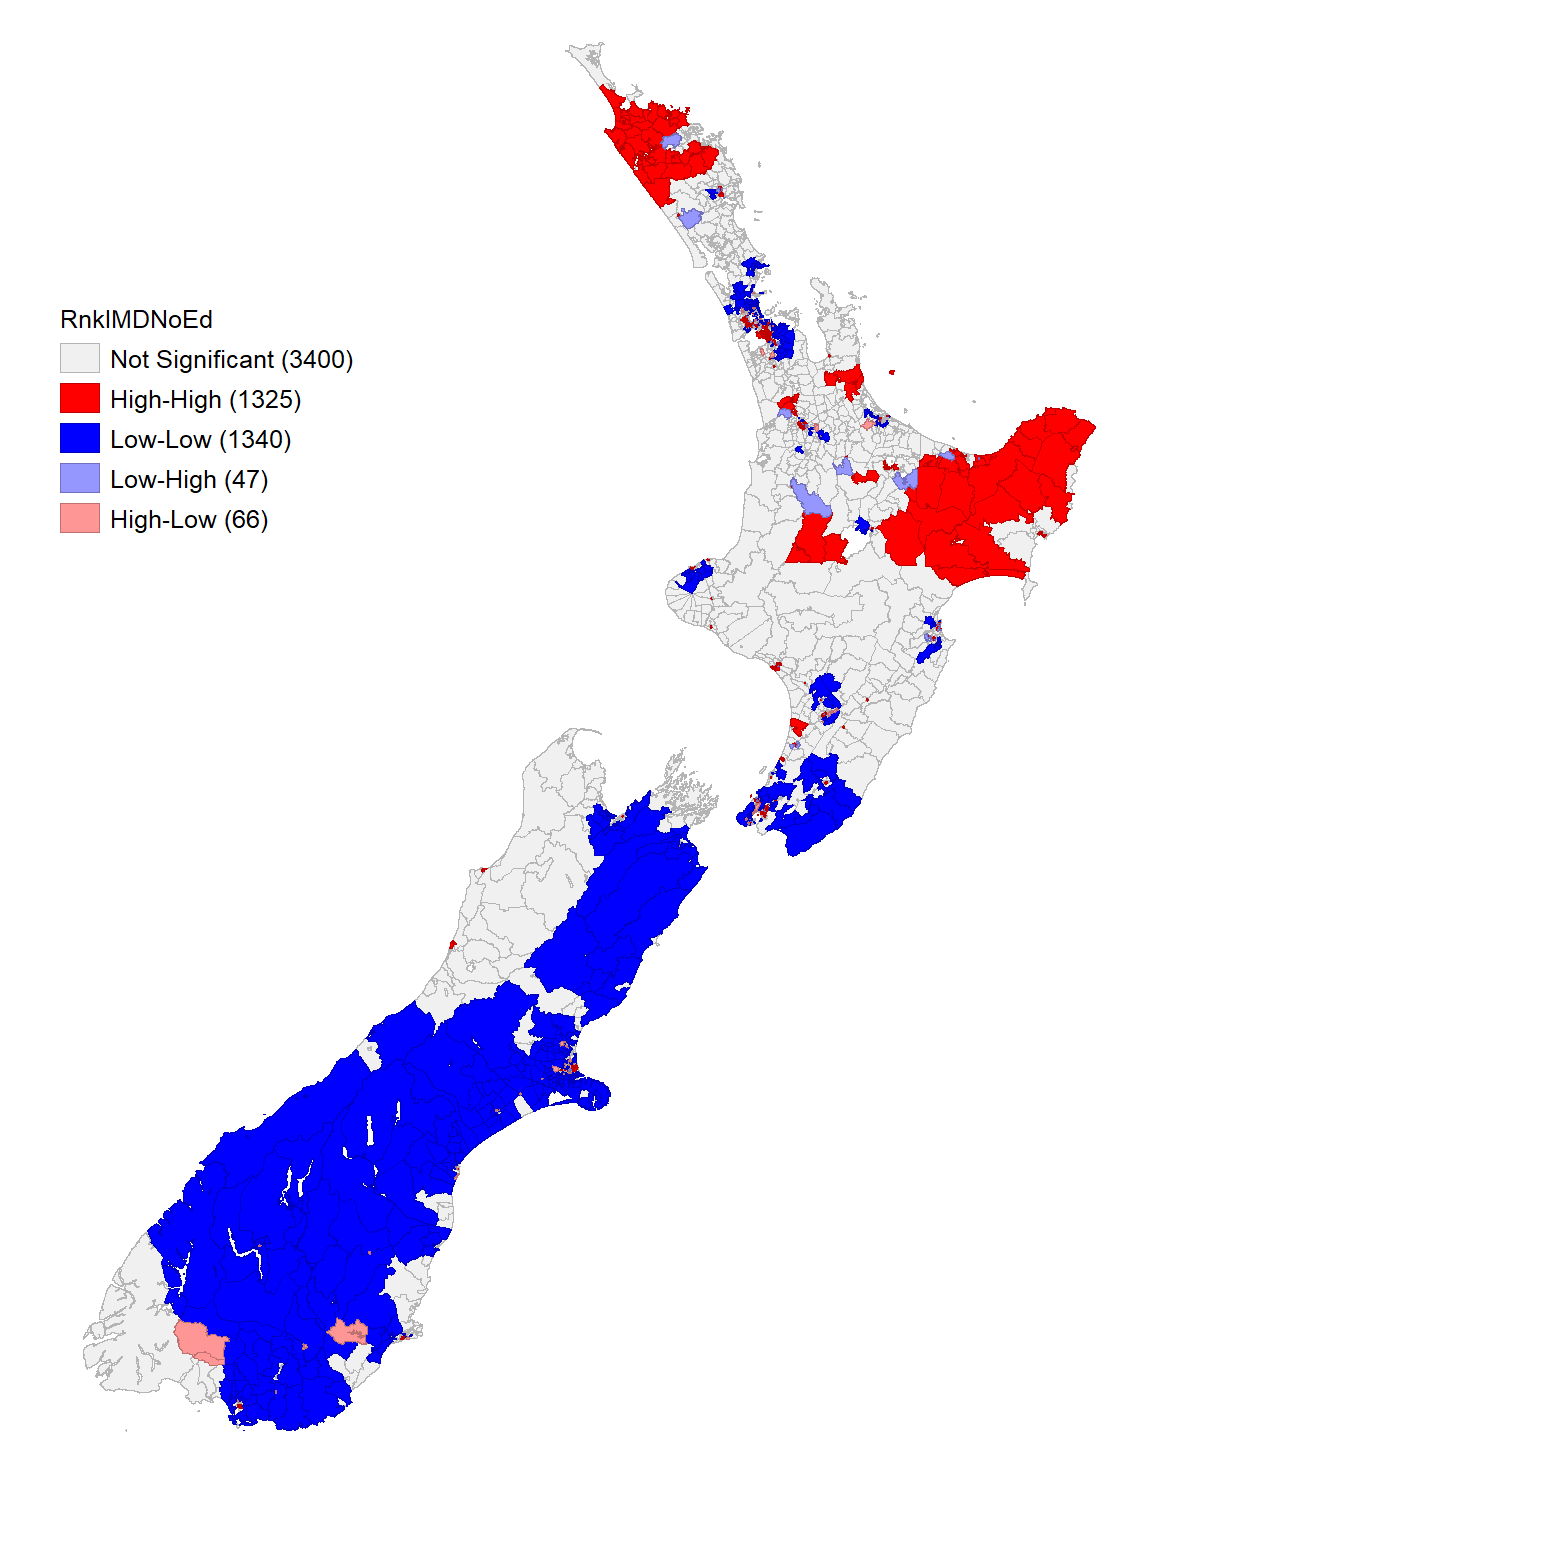
\includegraphics{imdnoed_localmoranI_uni_clustermap.png}

}

\caption{\label{fig-localiclusters}Local Moran's I cluster map from
GeoDa.}

\end{figure}

\begin{figure}

{\centering 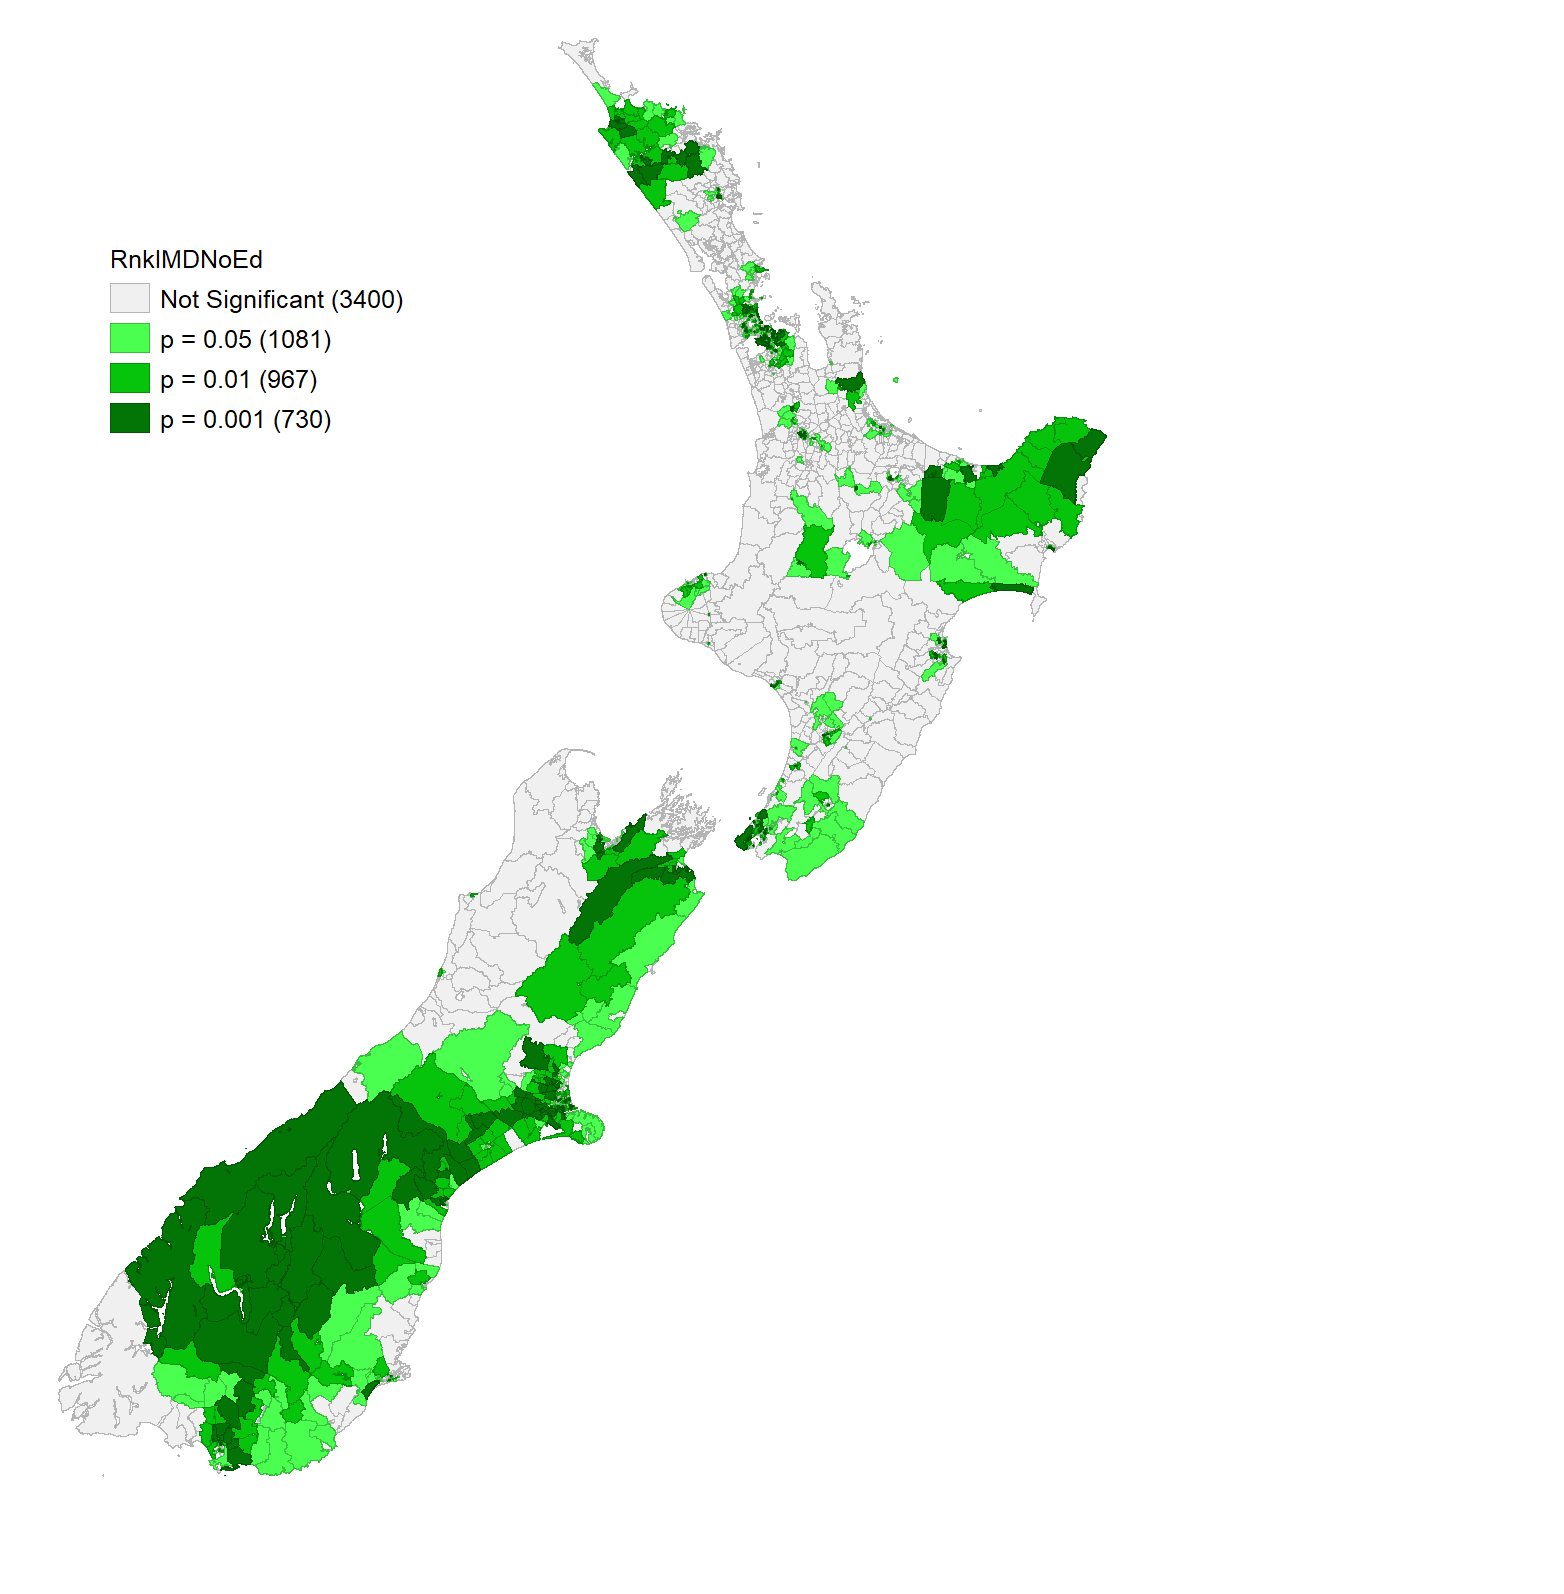
\includegraphics{imdnoed_localmoranI_uni_significance map.png}

}

\caption{\label{fig-localisig}Local Moran's I cluster significance map
from GeoDa.}

\end{figure}

\begin{figure}

{\centering 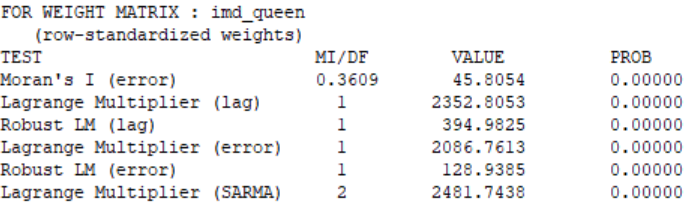
\includegraphics{Spatial model stuff.png}

}

\caption{\label{fig-spatial}Based on the Queen weight matrix, the
outputs and values of the Lagrange Multipliers for the final multiple
linear regression model.}

\end{figure}

\begin{figure}

{\centering 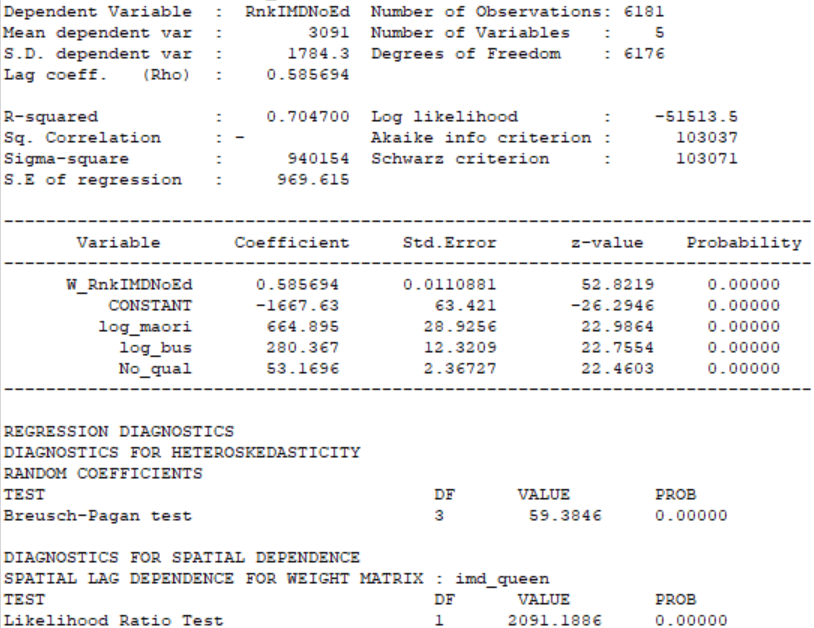
\includegraphics{Spatial lag regression.png}

}

\caption{\label{fig-spatiallag}Outputs of the Spatial Lag Linear
Regression model in GeoDa.}

\end{figure}

\hypertarget{works-cited}{%
\subsection*{Works Cited}\label{works-cited}}
\addcontentsline{toc}{subsection}{Works Cited}

\hypertarget{refs}{}
\begin{CSLReferences}{1}{0}
\leavevmode\vadjust pre{\hypertarget{ref-buxe9cares2013}{}}%
Bécares, Laia, Donna Cormack, and Ricci Harris. 2013. {``Ethnic Density
and Area Deprivation: Neighbourhood Effects on M{ā}ori Health and Racial
Discrimination in Aotearoa/New Zealand.''} \emph{Social Science \&
Medicine} 88 (July): 76--82.
\url{https://doi.org/10.1016/j.socscimed.2013.04.007}.

\leavevmode\vadjust pre{\hypertarget{ref-cooper2003}{}}%
Cooper, Mark, Lester Lloyd-Reason, and Stuart Wall. 2003. {``Social
Deprivation and Educational Underachievement: Lessons from London.''}
\emph{Education + Training} 45 (2): 79--88.
\url{https://doi.org/10.1108/00400910310464053}.

\leavevmode\vadjust pre{\hypertarget{ref-cutumisu2014}{}}%
Cutumisu, Nicoleta, Ariane Bélanger-Gravel, Marilie Laferté, François
Lagarde, Jean-Frédéric Lemay, and Lise Gauvin. 2014. {``Influence of
Area Deprivation and Perceived Neighbourhood Safety on Active Transport
to School Among Urban Quebec Preadolescents.''} \emph{Canadian Journal
of Public Health = Revue Canadienne de Santé Publique} 105 (5):
e376--82. \url{https://doi.org/10.17269/cjph.105.4561}.

\leavevmode\vadjust pre{\hypertarget{ref-exeter2018}{}}%
Exeter, Daniel John, Arier Chi Lun Lee, Jinfeng Zhao, Sue Crengle, Annie
Chiang, and Michael Browne. 2018. {``2018 Index of Multiple
Deprivation.''} \url{https://hgd.auckland.ac.nz/imd18/}.

\leavevmode\vadjust pre{\hypertarget{ref-shuttleworth1995}{}}%
Shuttleworth, Ian. 1995. {``The Relationship Between Social Deprivation,
as Measured by Individual Free School Meal Eligibility, and Educational
Attainment at GCSE in Northern Ireland: A Preliminary Investigation.''}
\emph{British Educational Research Journal} 21 (4): 487--504.
\url{https://doi.org/10.1080/0141192950210404}.

\leavevmode\vadjust pre{\hypertarget{ref-statsnz2020}{}}%
Stats NZ. 2020. {``2018 Census Place Summaries.''}
\url{https://www.stats.govt.nz/tools/2018-census-place-summaries/}.

\end{CSLReferences}



\end{document}
